\section{Methodology}
%\label{s:semantic-closeness}

In this work, we aim to utilize information from the semantic behavior of \cnc
to better control and guide the refinement process, producing a smaller
\abs while retaining the strong formal connection to \abs. 

In particular, we define a \textit{semantic
closeness metric} that captures how close the semantic behavior of two 
neurons is (Section \ref{s:semantic-closeness}). We utilize this semantic
closeness metric to arrange the merge
operations into a tree where the lower quality merges involving semantically far
neurons appear higher and can be refined with higher priority (Section
\ref{s:tree}). 

Using this tree, we build a framework where refinement can be
done by making cuts of this tree while still providing concrete soundness
guarantees (Section \ref{s:refinement}). We show that the merges retained in
this refinement process are optimal with respect to the semantic information 
(Section \ref{s:optimal-tree}). This allows us to avoid restoring a large
number of singleton neurons (see Section \ref{s:nn-sam}) and lets us retain merge 
operations of higher quality.

Using these components, we propose a general \cegar loop based
framework (Section \ref{s:abs-ref-fw}) that combines syntactic merge operations 
with semantic behavior. This framework is able produce an \abs strong enough to
not have any spurious counterexamples and with a much smaller size.

\subsection{Semantic Closeness Factor}
\label{s:semantic-closeness}

To guide the semantic abstraction process, we define a \emph{semantic
closeness metric} $\cls$: $\cls(\nr{i_1}{l}, \nr{i_2}{l})$ is a function that
takes two neurons $\nr{i_1}{l}$ and $\nr{i_2}{l}$ in
the same layer $l$, and returns a real number that
captures how close the behaviors of $\nr{i_1}{l}$ and $\nr{i_2}{l}$ are from a
semantic point of view. The number returned by $\cls$ should be smaller for
neurons whose semantic behavior is closer. Intuitively, this metric would
characterize the semantic behavior of the
neurons in layer $l$ relative to each other, and prioritize certain merges over
others. 

Depending on the application, the precise definition of this metric may be
chosen in various ways. We note that our framework is agnostic to the particular
choice of semantic metric, and the concrete soundness guarantee holds for any such
choice. Inspired by \cite{deep-abstract}, we choose the
semantic closeness metric to be the difference between the functions computed 
by the two neurons: $||\nrf{i_1}{l} - \nrf{i_2}{l}||_2$, where $|| \cdot ||_2$ is
the $L_2$ norm on the space of continuous functions on the input region $P
\subset \mathbb{R}^i \;{\rightarrow}\; \mathbb{R}$.
Generally, inputs to \dnn are bounded, and therefore so is $P$. 
Since $\nrf{i_1}{l}$ and $\nrf{i_2}{l}$ are neuron evaluations, they are
Lipschitz continuous \cite{nn-lipschitz},  which ensures that the $L_2$ norm is
well defined.

However, since computing
$||\nrf{i_1}{l} - \nrf{i_2}{l}||_2$ precisely is not feasible,
we estimate it using a sample set of inputs $X$: $||\ob{i_1}{l}($X$)
- \ob{i_2}{l}($X$)||_2$. In general this $X$ may be chosen in different ways,
and our framework is agnostic to the sampling strategy used. In our experiments,
we use a uniform sampling of the input region where $P$ holds. 
Since 
the input region is usually an interval, such sampling is
quite straightforward to do.

\subsection{Tree of Merges}
\label{s:tree}

We use $\cls$ to create a tree structure to prioritize merges where leaf nodes
represent the original neurons and non-leaf nodes represent merge operations. In
particular, each non-leaf node $m_i$ represents an operation merging all the neurons
corresponding to the leaf nodes that are descendants of $m_i$. For instance, 
the top half of Figure \ref{fig:Order_of_merging} shows a tree where $m_4$
merges $\nr{0}{1}$ and $\nr{1}{1}$, while $m_6$ merges $\nr{0}{1}$,
$\nr{1}{1}$, $\nr{2}{1}$ and $\nr{3}{1}$.

The construction of the tree follows a bottom-up approach, where we start from
individual neurons, and greedily perform the merge operation involving the most
similar groups of neurons, delaying the merging of dissimilar ones. This is
detailed in Algorithm \ref{a:build-tree} \footnote{ 
For our choice of $\cls$, (Section \ref{s:semantic-closeness}), Algorithm
\ref{a:build-tree} reduces to \hcluster, allowing us to leverage existing
efficient implementations. Nonetheless, the
general algorithm presented here will work for any choice of $\cls$.}:

We start with an initial structure
consisting only of leaf nodes corresponding to original neurons (line
\ref{a:build-tree:init}). At
this stage, no merge operation has yet been done, and each node is a potential
candidate for a merge, stored in $\cand$ at line
\ref{a:build-tree:init-cand}.

Now, as long as we have at-least two candidates that we can merge, we keep
greedily merging them in the loop starting at line \ref{a:build-tree:loop}. To
do this, we find which two candidate nodes $m_i$ and $m_j$ are most semantically
similar in line \ref{a:build-tree:get-mij}, and introduce an operation merging
them in lines \ref{a:build-tree:merge-start}-\ref{a:build-tree:merge-end}.

We measure how semantically close a pair of candidates $m_1$ and $m_2$ are by
looking at the maximum semantic distance between a neuron merged as a part of
$m_1$'s process and a that merged as a part of $m_2$'s process. This is done
recursively by the $\mathit{PairwiseMax}$ function in lines
\ref{a:build-tree:fn-start}-\ref{a:build-tree:fn-end}.

The resulting tree captures an optimal ordering of merge operations. 
That is, as we progress up the tree, the maximum value of $\cls$ between any two
neurons involved in a merge increases and the imprecision
introduced by the merge operation increases. 
This is formalized in Section \ref{s:optimal-tree}). 


\begin{algorithm}
\caption{Building the Tree}
\label{a:build-tree}
\begin{algorithmic}[1]

    \Require Neurons $\{\nr{i_1}{l}, {\cdots}, \nr{i_r}{l}\}$ with \inc-\dec
    label, Closeness metric $\cls$

    
    \State Initialize G with nodes $\{ \nr{i_1}{l}, {\cdots}, \nr{i_r}{l} \}$
    and no edges. \label{a:build-tree:init}

    \State Initialize $\cand=\{ \nr{i_1}{l}, {\cdots}, \nr{i_r}{l} \}$
    \label{a:build-tree:init-cand}

    \Function{PairwiseMax}{$m_1, m_2$} \label{a:build-tree:fn-start}
        
        \If{ $m_1$ or $m_2$ has children }
            \State Without loss of generality, say $m_1$ has children $c_1$ and
            $c_2$. 
            \State \textbf{return} $\max( PairwiseMax( c_1, m_2 ), PairwiseMax(
            c_2, m_2 ) )$
        \Else
            \State $m_1$ and $m_2$ are neurons, \textbf{return} $\cls( m_1, m_2 )$.
        \EndIf

    \EndFunction \label{a:build-tree:fn-end}

    \While{$|\cand|>1$} \label{a:build-tree:loop}
    
        \State $m_{j_1}, m_{j_2} = \arg\min_{\substack{m_1, m_2 \in \cand}} 
            \text{PairwiseMax}(m_1, m_2)$ \label{a:build-tree:get-mij}

        \State Add new node $m_{j_3}$ to $T$ \label{a:build-tree:merge-start}
        \State Make $m_{j_1}, m_{j_2}$ children of $m_{j_3}$ in $T$
        \State Remove $m_{j_1}, m_{j_2}$ from $\cand$ and add $m_{j_3}$ to
        $\cand$.
            \label{a:build-tree:merge-end}
    \EndWhile

    \State $G$ now is a tree, call it $T$

    \Ensure Tree of merges $T$
\end{algorithmic}
\end{algorithm}

As an example, consider the middle layer in Figure
\ref{fig:Original_Net_Property}. Here, $\nr{0}{1}$ and $\nr{1}{1}$ are
semantically closest. Thus, in the tree (top half of Figure
\ref{fig:Order_of_merging}), we first merge these two first to get the
node $m_4$, representing the merge group $\{\nr{0}{1}, \nr{1}{1}\}$. At this
point, we have three choices for the next merge operation: $m_4$ and
$\nr{2}{1}$, $m_4$ and $\nr{3}{1}$, or $\nr{2}{1}$ and $\nr{3}{1}$. Since
$\nr{2}{1}$ and $\nr{3}{1}$ are semantically closer to each other than to
$\nr{0}{1}$ or $\nr{1}{1}$, the algorithm merges
$\nr{2}{1}$ and $\nr{3}{1}$ to get $m_5$. This produces the merge group
$\{\nr{2}{1}, \nr{3}{1}\}$, which has elements that are semantically closer than
the groups $\{\nr{0}{1}, \nr{1}{1}\, \nr{2}{1}\}$ or $\{\nr{0}{1}, \nr{1}{1},
\nr{3}{1} \}$ obtained from following the other two choices. 
Finally, $m_4$ and $m_5$ get merged to $m_6$, giving us the complete tree.

\subsection{Tree-cuts and Refinement}
\label{s:refinement}



\begin{figure}[htbp]
    \centering
    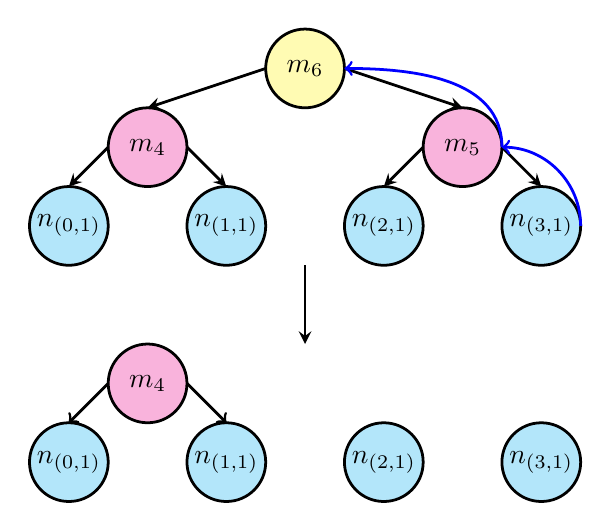
\begin{tikzpicture}[scale=0.5] % Adjust the scale factor as needed
        % Your TikZ code goes here
        \draw[line width=1pt,fill=yellow!30] (0,0) circle (1cm);
        \node at (0,0) {$m_6$};
        \draw[line width=1pt, fill=magenta!30] (-4,-2) circle (1cm);
        \node at (-4,-2) {$m_4$};
        \draw[line width=1pt, fill=magenta!30] (4,-2) circle (1cm);
        \node at (4,-2) {$m_5$};
        \draw[line width=1pt, fill=cyan!30] (-6,-4) circle (1cm);
        \node at (-6,-4) {$n_{(0,1)}$};
        \draw[line width=1pt, fill=cyan!30] (-2,-4) circle (1cm);
        \node at (-2,-4) {$n_{(1,1)}$};
        \draw[line width=1pt, fill=cyan!30] (6,-4) circle (1cm);
        \node at (6,-4) {$n_{(3,1)}$};
        \draw[line width=1pt, fill=cyan!30] (2,-4) circle (1cm);
        \node at (2,-4) {$n_{(2,1)}$};
        \draw[-> , >=stealth,line width=1pt] ({0 + cos(180)},{0 + sin(180)}) -- (-4,-1);
        \draw[->, >=stealth, line width=1pt] ({0 + cos(0)},{0 + sin(0)}) -- (4,-1);
        \draw[->, >=stealth, line width=1pt] ({-4 + cos(180)},{-2 + sin(180)}) -- (-6,-3);
        \draw[->, >=stealth, line width=1pt] ({-4 + cos(0)},{-2 + sin(0)}) -- (-2,-3);
        \draw[->, >=stealth, line width=1pt] ({4 + cos(180)},{-2 + sin(180)}) -- (2,-3);
        \draw[->, >=stealth, line width=1pt] ({4 + cos(0)},{-2 + sin(0)}) -- (6,-3);
        
        % Curved arrow
        \draw[->, color=blue, line width=1pt] (7, -4) to[out=90, in=0] (5, -2);
        \draw[->, color=blue, line width=1pt] (5, -2) to[out=90, in=0] (1, 0);
        \draw[->, >=stealth, line width=1pt] (0,-5) to (0,-7);

        \draw[line width=1pt, fill=magenta!30] (-4,-8) circle (1cm);
        \node at (-4,-8) {$m_4$};
        \draw[line width=1pt, fill=cyan!30] (-6,-10) circle (1cm);
        \node at (-6,-10) {$n_{(0,1)}$};
        \draw[line width=1pt, fill=cyan!30] (-2,-10) circle (1cm);
        \node at (-2,-10) {$n_{(1,1)}$};
        \draw[line width=1pt, fill=cyan!30] (6,-10) circle (1cm);
        \node at (6,-10) {$n_{(3,1)}$};
        \draw[line width=1pt, fill=cyan!30] (2,-10) circle (1cm);
        \node at (2,-10) {$n_{(2,1)}$};
    
        \draw[->, line width=1pt] ({-4 + cos(180)},{-8 + sin(180)}) -- (-6,-9);
        \draw[->, line width=1pt] ({-4 + cos(0)},{-8 + sin(0)}) -- (-2,-9);

    \end{tikzpicture}
    \caption{Trees and Cuts}
    \label{fig:Order_of_merging}
\end{figure}


In our abstraction refinement loop, we start with the fully merged network.
Then, whenever we get a \gencex $\vct{\beta}$, we
wish to refine the network. That is, we wish to choose which
neurons should remain merged. Intuitively, this choice should be guided
two factors: optimizing with respect to the semantic behavior of the network,
and attempting to eliminate $\vct{\beta}$. 

The tree produced in the previous Section \ref{s:tree} captures the semantic
behavior, and we use it to guide the refinement process as follows:
Any cut of the tree produces a set of trees. Then,  
the groups of neurons that we choose to keep merged correspond to the leaf nodes
of these trees. Therefore, finding a refinement reduces to finding cuts
in the tree.

To attempt to eliminate $\vct{\beta}$, we identify a \textit{culprit neuron}
$\gamma$ that contributes most to the spurious output on $\vct{\beta}$. The
intuition is that $\gamma$ should not be merged with any other neuron, as any
over-approximation of the behavior of $\gamma$ has a high chance of
introducing $\vct{\beta}$.

Thus, we do refinement in two steps. Firstly, we find the culprit neuron
$\gamma$. Then, we find a cut in the tree that ensures that $\gamma$ is not
merged with any other neuron.

\subsubsection{Finding $\gamma$}
\label{s:finding-gamma}

Many possible strategies may be used to identify the culprit neuron $\gamma$,
and our framework is agnostic to the specific strategy chosen. In our
experiments, the strategy we chose is based on the
\emph{gradient-guided refinement} described in \cite{lin-comb-abs-jan}. For each
potential $\gamma$ We calculate the following score, and chose $\gamma$ with the
largest score:

\begin{equation*}
\begin{aligned}
    \|v^{*}_{\gamma}(\vct{\beta}) - v_{\gamma}(\vct{\beta})\|_{2} \cdot 
    \big| \frac{\delta y(\vct{\beta})}{\delta v_{\gamma}} \big|
\end{aligned}
\end{equation*}

Here, 
$v_{\gamma}(\vct{\beta})$ is the value at the neuron $\gamma$ for input
$\vct{\beta}$ in the original \cnc, while $v^{*}_{\gamma}(\vct{\beta})$ is the
value of the neuron that $\gamma$ has been merged into within our current \abs.
$\frac{\delta y(\vct{\beta})}{\delta v_{\gamma}}$ is the partial derivative of
the output $y$ of \cnc with respect to the value at $\gamma$ for the input
$\vct{\beta}$.

\subsubsection{Cutting the Tree}

We wish to find a cut in the tree where $\gamma$ is not merged with any other
neuron, while also making sure that as many neurons remain merged as possible
(therefore minimizing the increase in size of \abs). To do this, we delete
precisely those nodes that are dependent on $\gamma$, starting from the parent
of $\gamma$ and moving up the tree following the parent links.

In our example, the culprit neuron is $\nr{3}{1}$. Thus, we traverse the tree
following the blue edges in Figure \ref{fig:Order_of_merging}, undoing $m_5$ and
$m_6$. This produces three trees, corresponding to leaving $\nr{0}{1}$ and
$\nr{1}{1}$ merged, while undoing the merge of $\nr{2}{1}$ and $\nr{3}{1}$.
Therefore, we get the \abs shown in Figure \ref{fig:tree_cut_refine}. Note
that in contrast to the refinement process followed by \cite{cegar-nn} (Section
\ref{s:nn-sam}), we retain merges of neurons that are semantically close
($\nr{0}{1}$ and $\nr{1}{1}$), avoid
proliferation of singletons, and achieve a smaller \abs that is sufficient to
prove the property in fewer iterations.

Once we have cut the tree and decided on which neurons to leave merged, the
actual merge operation is the exact same as that followed by \cite{cegar-nn}
(Section \ref{s:nn-sam}). Therefore, we are able to retain concrete soundness
guarantees.

\begin{figure}[htbp]
    \centering
    \begin{tikzpicture}[scale=0.5] % Adjust the scale factor as needed
      % Your TikZ code goes here
      \draw[fill=blue!30, line width = 1pt] (0,2) circle (1cm);
      \node at (0,2) {$n_{(0,0)}$};
      \node [text=red] at (-2,2) {1};
      \draw[fill=blue!30, line width = 1pt] (0,-2) circle (1cm);
      \node [text=red] at (-2,-2) {1};
      \node at (0,-2) {$n_{(1,0)}$};
      \draw[fill=orange!30, line width = 1pt] (5,4) circle (1cm);
      \node at (5,4) {$m_4$};
      \node [text=red] at (5,2.5) {1.5};
      \draw[fill=pink!30, line width = 1pt] (5,-4) circle (1cm);
      \node at (5,-4) {$n_{(3,1)}$};
      \node [text=red] at (5,-5.5) {1.5};
      \draw[fill=pink!30, line width = 1pt] (5,0) circle (1cm);
      \node at (5,0) {$n_{(2,1)}$};
      \node [text=red] at (5,-1.5) {1.9};
      \draw[fill=green!30, line width = 1pt] (10,0) circle (1cm);
      \node at (10,0) {$n_{(0,2)}$};
      \node [text=red] at (12,0) {$6.8$};
    \draw[->, >= angle 45, line width = 1pt, postaction={decorate, decoration={text along path, 
    text={0.55}, text align=center, raise=1mm}}](1, 2) -- (4, 4);
    \draw[->,>= angle 45, line width = 1pt] (1, -2) to (4, 4);
    \node at (3.75,3) {1};
    \draw[->,>= angle 45, line width = 1pt](1, 2) -- (4, 0);
    \node at (3.75,1) {0.95};
    \draw[->,>= angle 45, line width = 1pt](1, -2) -- (4, 0);
    \node at (3.75,-1) {0.55};
    \draw[->,>= angle 45, line width = 1pt](1, 2) -- (4, -4);
    \node at (3.75,-3) {1};
    \draw[->, >= angle 45, line width = 1pt, postaction={decorate, decoration={text along path, 
    text={0.5}, text align=center, raise=1mm}}](1, -2) -- (4, -4);
    \draw[-> , >= angle 45, line width = 1pt, postaction={decorate, decoration={text along path,
    text={1}, text align=center, raise=1mm}}] (6,-4) -- (9, 0);
    \draw[->, >= angle 45, line width = 1pt, postaction={decorate, decoration={text along path,
    text={1}, text align=center, raise=1mm}}] (6,0) -- (9, 0);
    \draw[->, >= angle 45, line width = 1pt, postaction={decorate, decoration={text along path,
    text={2}, text align=center, raise=1mm}}] (6,4) -- (9, 0);
   
    % \draw (1, -2) -- (4, 2);
    % \node at (3.75,1.25) {1};
  
    % \draw (1, 2) -- (4, -2);
    % \node at (3.75,-1.25) {1};
  
    % \draw[solid, postaction={decorate, decoration={text along path,
    % text={0.95}, text align=center, raise=1mm}}] (1, 2) -- (4, 2);
   


    % \draw[solid, postaction={decorate, decoration={text along path,
    % text={1}, text align=center, raise=1mm}}] (6,-2) -- (9, 0);
    % \draw[solid, postaction={decorate, decoration={text along path,
    % text={3}, text align=center, raise=1mm}}] (6, 2) -- (9, 0);

    \end{tikzpicture}
    \caption{Refining by our method: Culprit Neuron is 3 }
    \label{fig:tree_cut_refine}
  \end{figure}
  


\subsection{Optimality of Tree}
\label{s:optimal-tree}

\textbf{Notation:} Given a (sub)tree $T$ of
merge operations, we say a neuron $\nr{i}{l} \in T$ if and only if $T$ has a
leaf node corresponding to $\nr{i}{l}$. That is, $\nr{i}{l} \in T$ if and only
if the merge operations forming $T$ involve $\nr{i}{l}$ at any point.

The tree $T$ produced in Section \ref{s:tree} captures an optimal ordering of
merge operations with respect to the semantic information in the following
sense:

\begin{lemma}
Let $T_1$ and $T_2$ be two sub-trees of $T$. Then, we have:

\begin{equation*}
\begin{aligned}
    \max_{ \substack{ \nr{i_1}{l} \in T_1 \\ \nr{i_1'}{l} \in T_1 }} 
    \cls( \nr{i_1}{l}, \nr{i_1'}{l} ) \leq
    \max_{ \substack{ \nr{i_1}{l} \in T_1 \\ \nr{i_2}{l} \in T_2 }} 
    \cls( \nr{i_1}{l}, \nr{i_2}{l} )
\end{aligned}
\end{equation*}

%the maximum value of $\cls$
%for any two neurons that are leaves $T_1$ (or $T_2$) is smaller than the maximum
%value of $\cls$ for any two neurons one from $T_1$ and another from $T_2$.
\end{lemma}
\begin{proof}
This fact can be easily proved via induction on the combined size of $T_1$ and
$T_2$. If a violation to the inequality exists, there may be two cases. In the
first case, we have $\nr{i_1}{l}, \nr{i_1'}{l} \in T_1'$ where $T_1'$ is a
strict sub-tree of $T_1$. But$T_1'$ and $T_2$ would then form a violation of the
induction hypothesis. The other case directly violates the pairwise maximum
condition  used in the construction of the
tree in Algorithm \ref{a:build-tree} line \ref{a:build-tree:fn-start}
in Section \ref{s:tree}.
\end{proof}

Intuitively, the lemma shows that for any cut in the tree, the
maximum difference in the semantic behavior of neurons that have been left
merged is less than the maximum difference in the semantic behavior of neurons
that have been un-merged. In particular, this implies that after each refinement
step, the groups of neurons that remain merged together are optimal with respect
to the semantic behavior of the network.

However, note that our semantic closeness metric fails to say anything about the
value produced at the output layer of the network for any given input. Thus,
although we have optimality with respect to semantic behavior, we are unable to
predict the result making a cut would have on the output for the given \gencex.
Attempting to make such a prediction, or provide some guarantees on the output
of the network for a given spurious input, would nonetheless be an interesting
direction for future work.

\subsection{\cegar Loop Framework}
\label{s:abs-ref-fw}

We combine the pieces discussed so far into a \cegar loop.  
We start with the fully merged network. Then, utilizing \gencex, we iteratively
refine the network until we have obtained an \abs where there is no \gencex.
This loop is parametrized by:

\begin{itemize}
    \item The definition of the semantic closeness factor $\cls$.
    \item The strategy for selecting the culprit neuron $\gamma$.
\end{itemize}

We note that while we have provided specific strategies for each of these, our
framework is flexible enough so that, depending on the application, these pieces
may be swapped out or modified to achieve better performance. We intend to study
other strategies for each of these pieces in the future.
